
\section{Turbulent boundary layers under adverse pressure gradients}

A wall-bounded flow can be subjected to pressure gradients as a result of the curvature of the wall, but also as a result of a change in the direction/velocity components at the boundary-layer edge.
Turbulence is already a complex problem in a ZPG case with the only parameter being the Reynolds number. If another parameter such as pressure gradients is added, the complexity of the problem increases and it becomes difficult to distinguish what phenomena is caused by the $\Rey$ effects or by the PG history of the flow \citep{bobke2017}.
In order to properly study APG TBLs, first we should try to define a canonical simple case consisting of a well-defined APG along the streamwise development of the TBL. 
\rev{this is what we refer as the PG history of the flow.}
Different parameters have been used to quantify the pressure-gradient magnitude in literature, such as the Rotta-Clauser PG parameter $\beta$, or a general $\Lambda_{\mathrm{inc}}$ which in \cite{Gibis2019} is studied with different length and velocity scales.
In our simulations of moderate APGs we have used $\beta$ defined as:
\begin{equation}
    \beta(x) = \frac{\delta^*}{\tau_w} \pdv{P_e}{x},
\end{equation}
where $\pdv{P_e}/{x}$ is the average streamwise pressure gradient at the boundary-layer edge, $\tau_w$ is the mean wall-shear stress, and $\delta^*$ is the displacement thickness, which for an incompressible flow is defined as:
\begin{equation}
    \label{eq:dstar_cap3}
    U_e \delta^* = \int_{0}^{\delta_{99}} (U_e - U) \mathrm{d}y.
\end{equation}
% IDEA behind beta
Note that in Eq.~(\ref{eq:dstar_cap3}) we truncate the integration in $y$ at $\delta_{99}$ due to the nonzero velocity gradient induced by the pressure gradient~\citep{diagnostic_Vinuesa}. The idea behind the $\beta$ parameter is to stablish an integral equilibrium of forces across the TBL, in this way, every section of the TBL is subjected to the same dimensionless state of forces.
This is reflected in Fig.~\ref{fig:scheme_beta}, which shows a schematic representation  of a section of the BL, where the main forces are due to the streamwise pressure gradient and the wall-shear stress.

\begin{figure}
    \centering
    \includegraphics[width=0.90\textwidth]{imgs/schemes/scheme_beta.jpg}
    \caption{Stresses around a section of a BL.}
    \label{fig:scheme_beta}
\end{figure}

Integrating the streamwise momentum equation over the wall-normal direction, under several assumptions, it is possible to obtain an equation which relates the integral parameters $\delta^*$, $\theta$ (which is the momentum thickness) and $\beta$. Thus, from an integral approach, the thickness $\delta \myprime$ is chosen equal to $\delta^*$. 


\section{Turbulence statistics}
In \textbf{Paper 1} we explore the statistical quantities of TBLs under APGs. The novelty with respect to the available literature was in the high-fidelity database used for the ZPG and APG TBLs. Both simulations show the development of the TBL from low Reynolds numbers such as those of previous numerical databases, and reach large Reynolds numbers such as those obtained in experiments. This characteristic works as a bridge to validate previous simulations as well as the current simulations, since they have been compared successfully with experimental data.
A benefit of numerical data over experiments is the higher availability of data, which enables better measurements close to the wall.

\begin{table}
  \begin{center}
  \fontsize{8.0pt}{10.25pt}\selectfont
  \addtolength{\tabcolsep}{-2pt}
\def~{\hphantom{0}}
    \begin{tabular}{ l c  r }
    Case  & Colour & Reference \\[3pt]
    \hline
    b1             & \redline     & Bobke {\it et al.}(\citeyear{bobke2017}) \\
    b2             & \greenline   & Bobke {\it et al.}(\citeyear{bobke2017}) \\
    m16            & \blueline    & Bobke {\it et al.}(\citeyear{Bobke_2016}) \\

    ZPG            & \blackline   & Eitel-Amor {\it et al.}(\citeyear{EAmorZPG}) \\
    b1.4           & \orangeline  & Pozuelo {\it et al.}(\citeyear{Pozuelo_JFM_22}) \\
    exp            & \redcircle   & Sanmiguel Vila {\it et al.}(\citeyear{MTL_expSANMIGUEL}) \\
    \hline
    \end{tabular}
  \caption{ Line styles and colors for the simulations and experiments used in the thesis.}
  \label{tab:param_cap2}
  \end{center}
\end{table}

In Fig.~\ref{fig:U_uu_cap2}(a) we show the inner-scaled $U$ and $\sqrt{\overline{u\myprime u\myprime}} = u_{\mathrm{rms}}$ for various TBLs (see Table~\ref{tab:param_cap2}) at $\Rey_{\tau}=500$, where the low-Reynolds-number simulations are already fully turbulent. At the higher $\Rey_{\tau}=2100$ we also have an experimental near-equilibrium APG TBL, and both the ZPG simulation by \cite{EAmorZPG} and our new APG simulation (b1.4)~\citep{Pozuelo_JFM_22} are at a similar Reynolds number.
The experimental data \citep{MTL_expSANMIGUEL} and the b1.4 case are in a similar range of $\beta$ and their statistics exhibit a good agreement in the streamwise mean and fluctuating velocity components. Note that here `+' denotes inner scaling, {\it i.e.} in terms of the friction velocity $u_{\tau}$ or the viscous length $\ell_{\tau}=\nu/u_{\tau}$.
The APG leads to a lower $U^+$ for larger $\beta$ in the logarithmic region, and a larger effect in the wake region. At higher Reynolds numbers, the logarithmic region grows and the near-equilibrium APG and the ZPG profiles get closer because of the smaller effect of APGs for increasing $Re$~\citep{Vinuesa_2017, vinu18b}.

In the turbulent perturbations, the near-wall or inner peak of $u_{\rm rms}$, which
we will denote with the subindex `IP', grows in value with both the Reynolds number and the APG effects and its wall-normal position $y_{\rm IP}^+$ appears to slightly increase with both APG and $\Rey$ effects~\citep{Pozuelo_JFM_22}.

Higher Reynolds numbers allow for larger scales to live in the logarithmic/wake region and for a larger separation of the scales to be seen. This is first seen as lower decay in $u_{\rm rms}$ in the ZPG case within the logarithmic/wake region and a development of an outer peak for APG profiles. Larger $\beta$ values increase the magnitude of the outer peak of $u_{\rm rms}$. The trends for the outer-peak value and wall-normal position of the RS,  $\overline{u\myprime^2}_{\rm OP}$ and $y_{\rm OP}$ where analysed in \cite{Pozuelo_JFM_22}. 


\begin{figure}
    \centering
    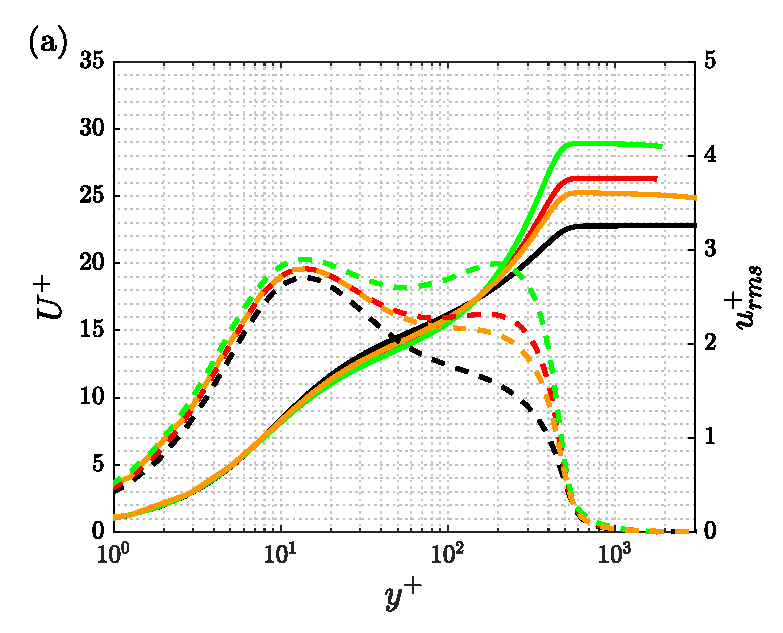
\includegraphics[width=0.49\textwidth]{imgs/stats/U_uu_a.eps}
    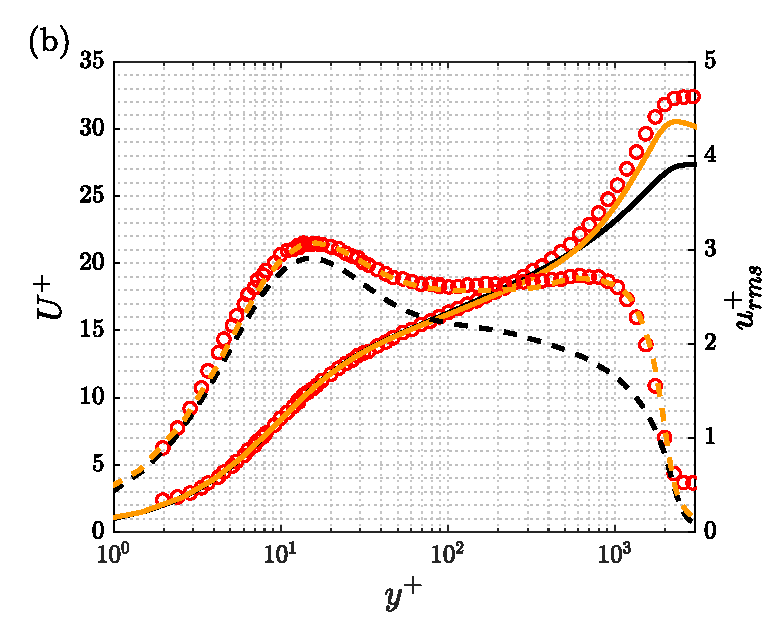
\includegraphics[width=0.49\textwidth]{imgs/stats/U_uu_b.eps}
    \caption{Inner-scaled streamwise mean velocity (solid lines) and root-mean-squared streamwise velocity (dashed lines) as a function of the inner-scaled wall-normal location for (a) $\Rey_{\tau}=500$ and (b) $\Rey_{\tau}=2100$. }
    \label{fig:U_uu_cap2}
\end{figure}

\subsection{Skin-friction coefficient $c_f$}

The drag in aerodynamic structures has an important contribution from the friction at the wall, also known as skin friction, which is the mean shear stress produced at the wall due to the viscous forces.
Instead of the wall-shear stress $\tau_w$, it is common to look at the skin-friction coefficient $c_f$, which is a ratio between the friction stresses and the free flow:
\begin{equation}
    \label{eq:cf_cap3}
    c_f = \frac{\tau_w}{1/2 \rho U_e^2} = 2\left( \frac{u_{\tau}}{U_e} \right)^2 .
\end{equation}
Note that $c_f$ can also be seen as an indicator of the friction velocity with respect to the freestream velocity, as shown in Eq.~(\ref{eq:cf_cap3}).
\begin{figure}
    \centering
    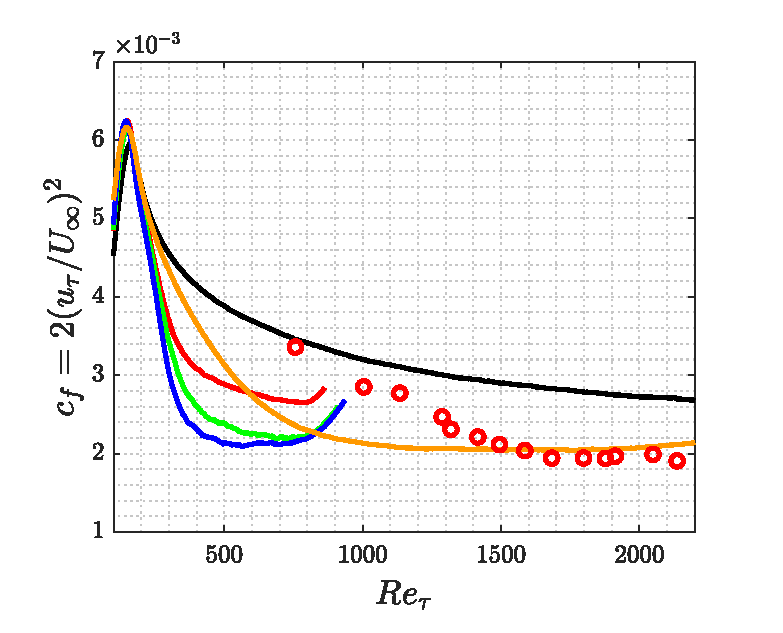
\includegraphics[width=0.85\textwidth]{imgs/stats/cf_Retau.eps}
    \caption{Evolution of the mean skin-friction coefficient for ZPG and APG simulations (solid lines) and experiments by \cite{MTL_expSANMIGUEL} (red circles). See Table~\ref{tab:param_cap2} for interpretation of the colors.}
    \label{fig:cap3_evol_cf}
\end{figure}
In Fig.~\ref{fig:cap3_evol_cf} we show the streamwise development of the skin-friction coefficient in boundary layers from ZPG and APG simulations, as well as that of an experimental APG.
It can be seen how for attached flows and near-equilibrium TBLs the trend is positive, decays with the Reynolds number and the value is lower the stronger the APG intensity.
The simulations show a mild increase for the larger $\Rey_{\tau}$ where the fringe region starts to affect the flow, and this region is not included in the region of interest (ROI) of our database.
Note that the effects of APG on $c_f$ are studied through the Renard--Deck (RD) \citep{Renard2016} identity in \textbf{Paper 3} and the Fukagata--Iwamoto--Kasagi identity (FIK) \citep{Fukagata2002} in \textbf{Paper 4}.

The FIK decomposition of $c_f$ is adapted to include a joint contribution of the pressure gradient and the streamwise convection from a dynamic-pressure perspective, instead of treating these contributions as separate entities.
A different perspective to the analysis of $c_f$ is that of the RD decomposition, taken from a perspective based on the mean streamwise kinetic energy budget. 
The main contributions to the total $c_f$ are divided into three main terms representing the viscous dissipation, the turbulent kinetic energy production and the spatial growth.
The contribution from the viscous diffusion is mainly located in the inner/near-wall region of the TBL and the influence diminishes for stronger APGs, since larger scales located in the outer region of the TBL are more energized and their effects on $c_f$ are more prominent.
The TKE production close to the wall has a near-wall peak that influences $c_f$, but the impact of the APG also produces a strong outer-peak in the outer region.
The spatial-growth contribution is further decomposed into three subterms, and the main ones are due to the mean convection $\mathbf{U}\cdot \nabla\mathbf{U}$ (which has a positive contribution across the TBL) and a direct contribution of the pressure gradient (which has a negative contribution on $c_f$). These terms are more relevant for stronger APGs and decrease with $\Rey$. Also note that their influence is mostly located in the outer region of the TBL.


\section{Spectral decomposition}
To have a better understanding on the perturbations we can use some mathematical tools such as the decomposition of the spatio-temporal signal using correlations, orthogonal modes, coherent structures, etc.
The use of orthogonal modes allows to decompose the energy of the perturbations into each mode in an unique way, so the sum of the energy contained in all the modes is equivalent to the total energy of the perturbations. 

In signal analysis an orthogonal decomposition which is commonly used is the Fourier decomposition which enables to analyze phenomena that repeat their behavior with some temporal and/or spatial frequencies. The energy or power associated with each mode is called energy spectrum (if the signal is finite in time, such as the case of pulses) or power spectrum (if the signal is not finite in time; in this case its temporal domain and energy are not finite, but its power is). We recall that the power is the ratio of the energy over time, where the time goes to infinity (in the case of using temporal series).
Since we are dealing with signals which are periodic in the homogeneous dimension $z$ and are not limited in time, we will use the terminology of power spectrum (PS) instead of energy spectrum. 
The modes in $z$ have a wavenumber $k_z$ and a wavelength $\lambda_z=2\pi/L_z$ where $L_z$ is the spanwise period of the domain. The same analysis can be applied in time, where we will use $k_t$ and $\lambda_t$.
For a signal $x(t)$, with $X(k_t)$ being its Fourier transform, the power of each mode is $|X(k_z)|^2$, {\it i.e.} the squared amplitude of the mode. For a perturbation velocity, the power can be calculated as:
\begin{equation}
    \mathrm{PS}_{u_i\myprime u_j\myprime}(k_z) = \mathcal{F}(u_i \myprime)  \mathcal{F}^*(u_j \myprime),
    \label{eq:power_sp}
\end{equation}
where $\mathcal{F}()$ is the Fourier transform and $\mathcal{F}^*()$ represents the complex conjugate and the definition has been expanded to include the power spectrum of the quantity $\langle u_i\myprime u_j\myprime \rangle_{z}$, also known as cospectrum.
Using the properties of the Fourier transform, the multiplication in Fourier space represented in Eq.~(\ref{eq:power_sp}) represents the Fourier transform of the two-point correlation function $\mathcal{R}_{u_i\myprime, u_j\myprime}(\delta z)=u_i\myprime \star u_j\myprime$, where $\delta z$ is the lag or distance between the two points where we assess the correlation of their velocity perturbations. According to the Wiener--Khinchin theorem, we can calculate the PS as the Fourier transform of $\mathcal{R}_{u_i\myprime, u_j\myprime}$, and it is possible to obtain the two-point correlation function from the power spectrum through the inverse Fourier transform $\mathcal{F}^{-1}()$.

Note that for velocity perturbations, since Fourier modes are orthogonal, the sum of the PS for all the modes is equal to the averaged Reynolds stress:
\begin{equation}
    \label{eq:sum_PS_cap3}
    \langle u_i\myprime u_j\myprime \rangle_{z} = \sum_{k_z} \mathrm{PS}_{u_i\myprime u_j\myprime}(k_z).
\end{equation}
This step can be performed for each time step and averaged over time to obtain $\langle\langle u_i\myprime u_j\myprime \rangle_{z}\rangle_{t} = \overline{u_i\myprime u_j\myprime}$ or it can also be the result of a 2D spectral decomposition in both time and $z$, where the sum extends to all the spatial and temporal modes.
The PS is useful for discrete systems, and it is the first step when we calculate the spectrum of the Reynolds stresses. It is also interesting to see how the power spectrum is distributed along the wavenumbers or the wavelengths, obtaining the power-spectral density (PSD).
The average in time of the PSD in wavenumbers is $\phi_{u_i\myprime u_j\myprime}=\langle \mathrm{PS} \rangle_t/\mathrm{d} k_z$ while the PSD averaged in time for the wavelengths is $\psi_{u_i\myprime u_j\myprime}= \langle \mathrm{PS} \rangle_t/\mathrm{d} \lambda_z$. Both densities can be linked using $\mathrm{d}(\lambda_z) = \mathrm{d}(2\pi/k_z) = -2\pi\mathrm{d}k_z/k_z^2$:

\begin{equation}
    \psi_{u_i\myprime u_j\myprime} = 
    \frac{ \langle \mathrm{PS}_{u_i\myprime u_j\myprime} \rangle_t}{\mathrm{d} \lambda_z} =
    -\frac{ \langle \mathrm{PS}_{u_i\myprime u_j\myprime} \rangle_t}{\mathrm{d} k_z} \frac{k_z^2}{2\pi}=
    \highlight{-\phi_{u_i\myprime u_j\myprime} \frac{k_z^2}{2\pi},}
\end{equation}
where the minus sign accounts for inverting the limits of integration to obtain the total RS (integrating from small to large wavenumbers is equivalent to integrating from large to small wavelengths):

\begin{equation}
\label{eq:sum_ps}
    \overline{u_i\myprime u_j\myprime} = 
    \int_{k_z=k_0}^{k_z=k_{N}}   \phi_{u_i\myprime u_j\myprime}  ~ \mathrm{d} k_z =
    \int^{\lambda_z = 2\pi/k_0}_{\lambda_z = 2\pi/k_{N}}  \psi_{u_i\myprime u_j\myprime}  ~ \mathrm{d} \lambda_z.
\end{equation}

\begin{figure}[h!]
\centering
% \captionsetup{width=0.99 \textwidth}
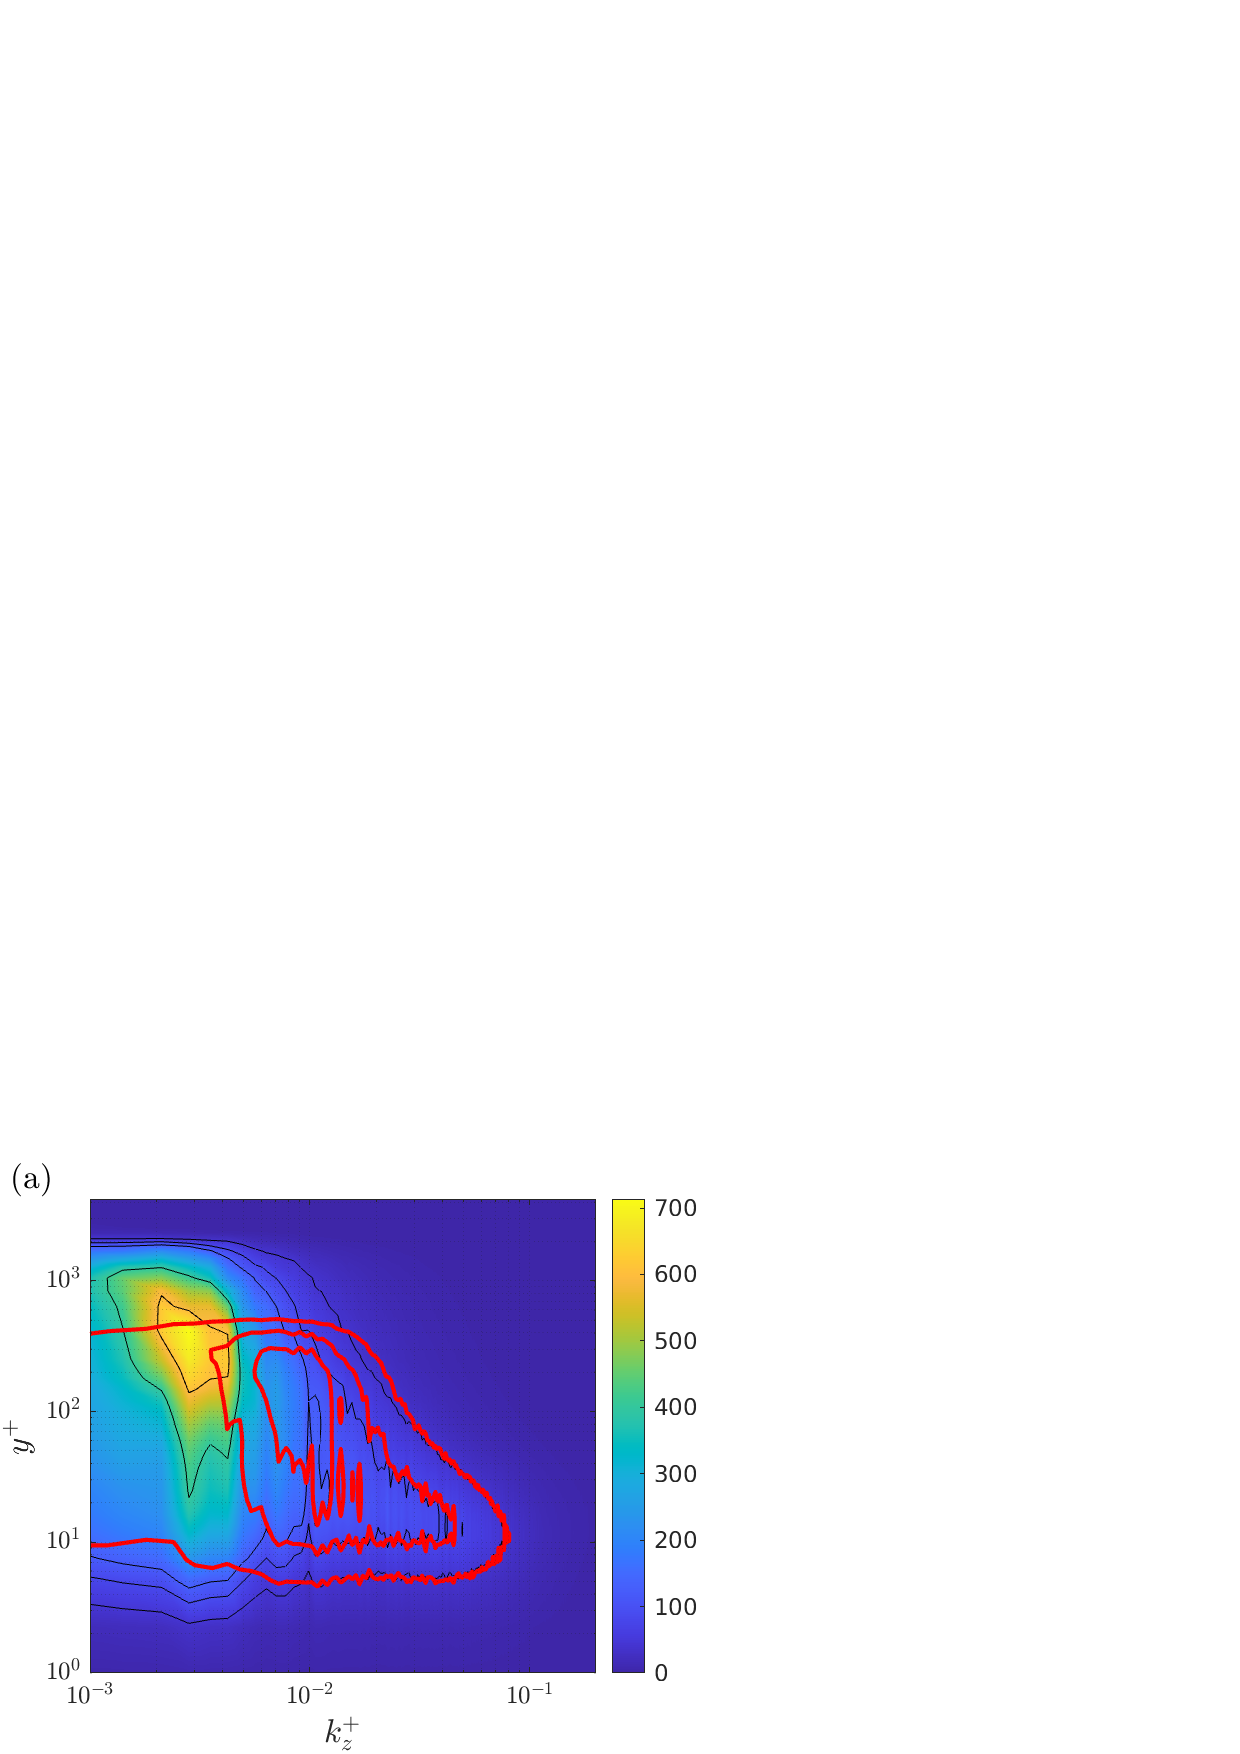
\includegraphics[width=0.32\textwidth ]{imgs/spec/ZPG_Ret_500_2000_PSdkz_kz_ltau_y_ltau.jpg}
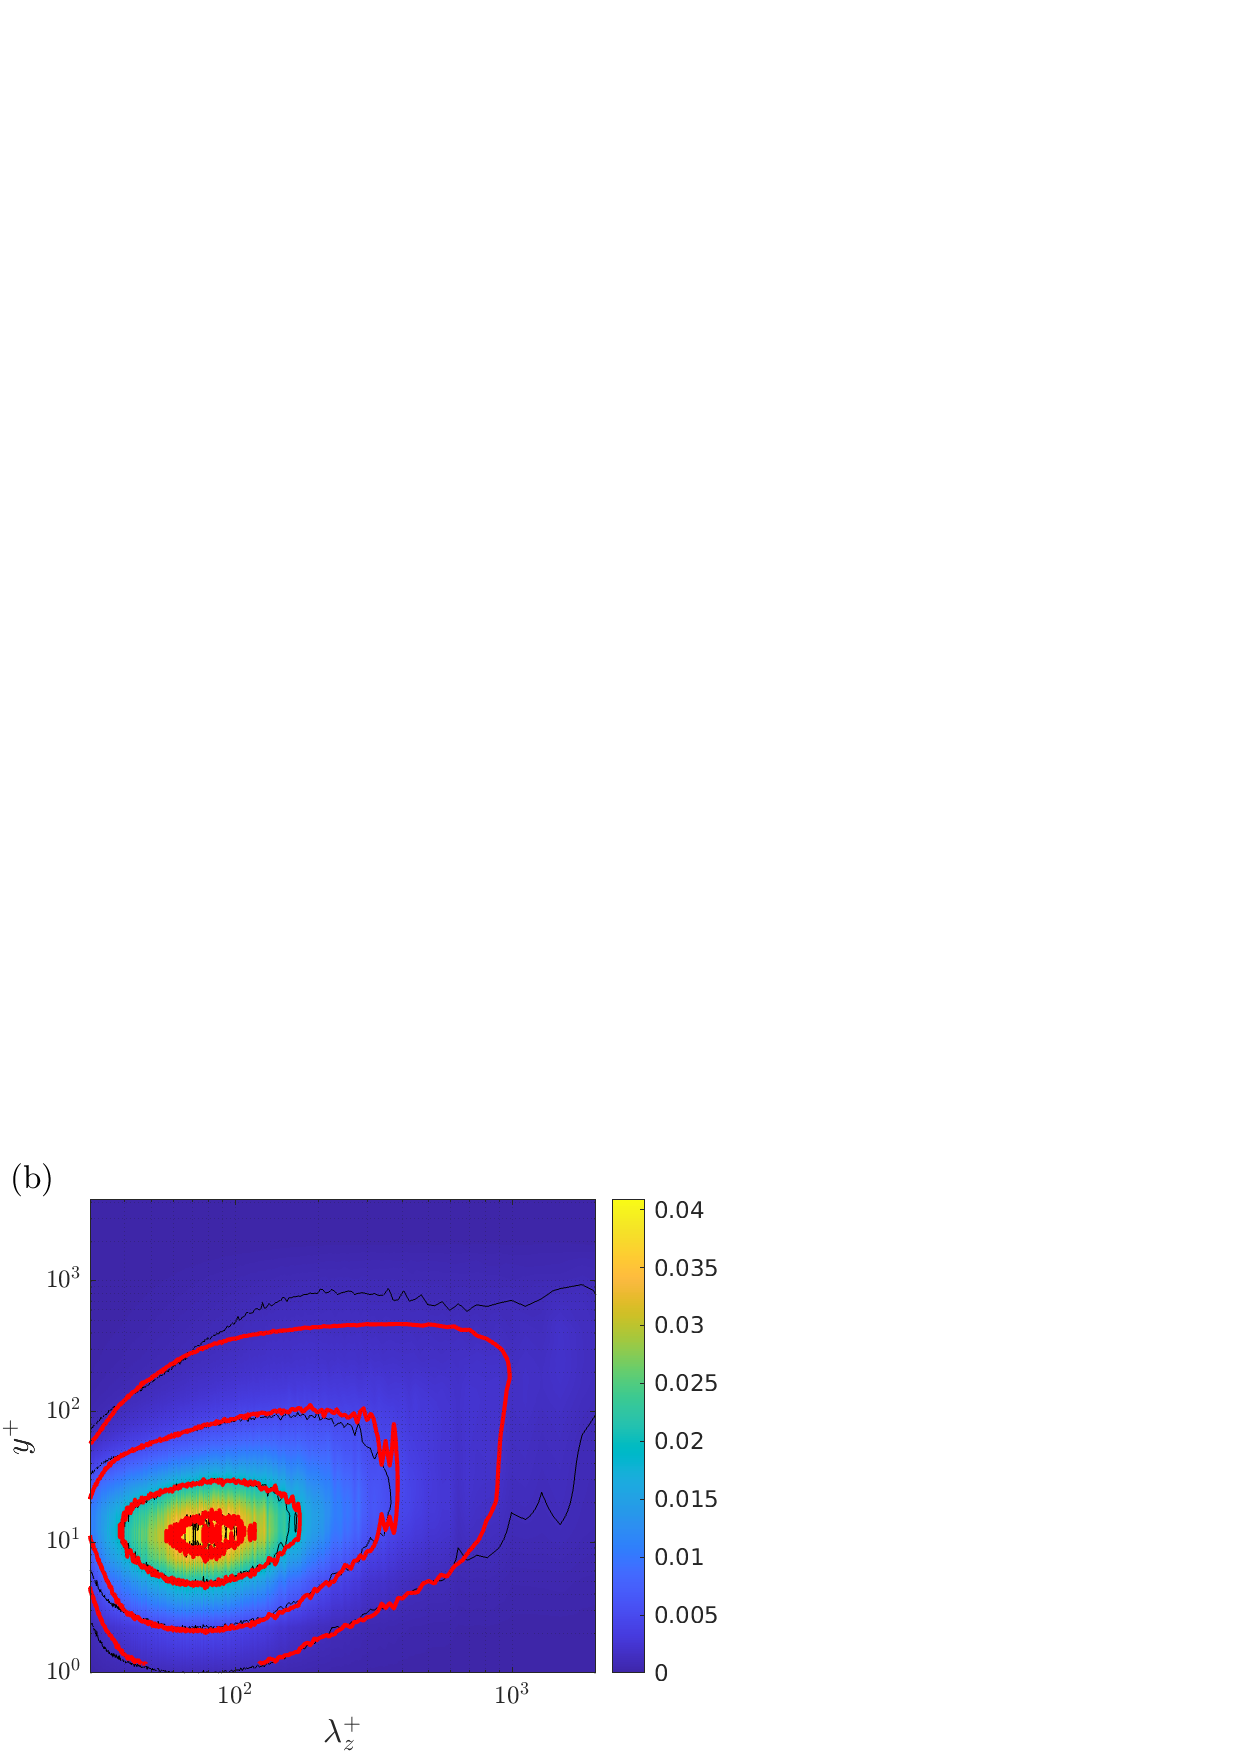
\includegraphics[width=0.32\textwidth]{imgs/spec/ZPG_Ret_500_2000_PSdlambdaz_lambdaz_ltau_y_ltau.jpg}
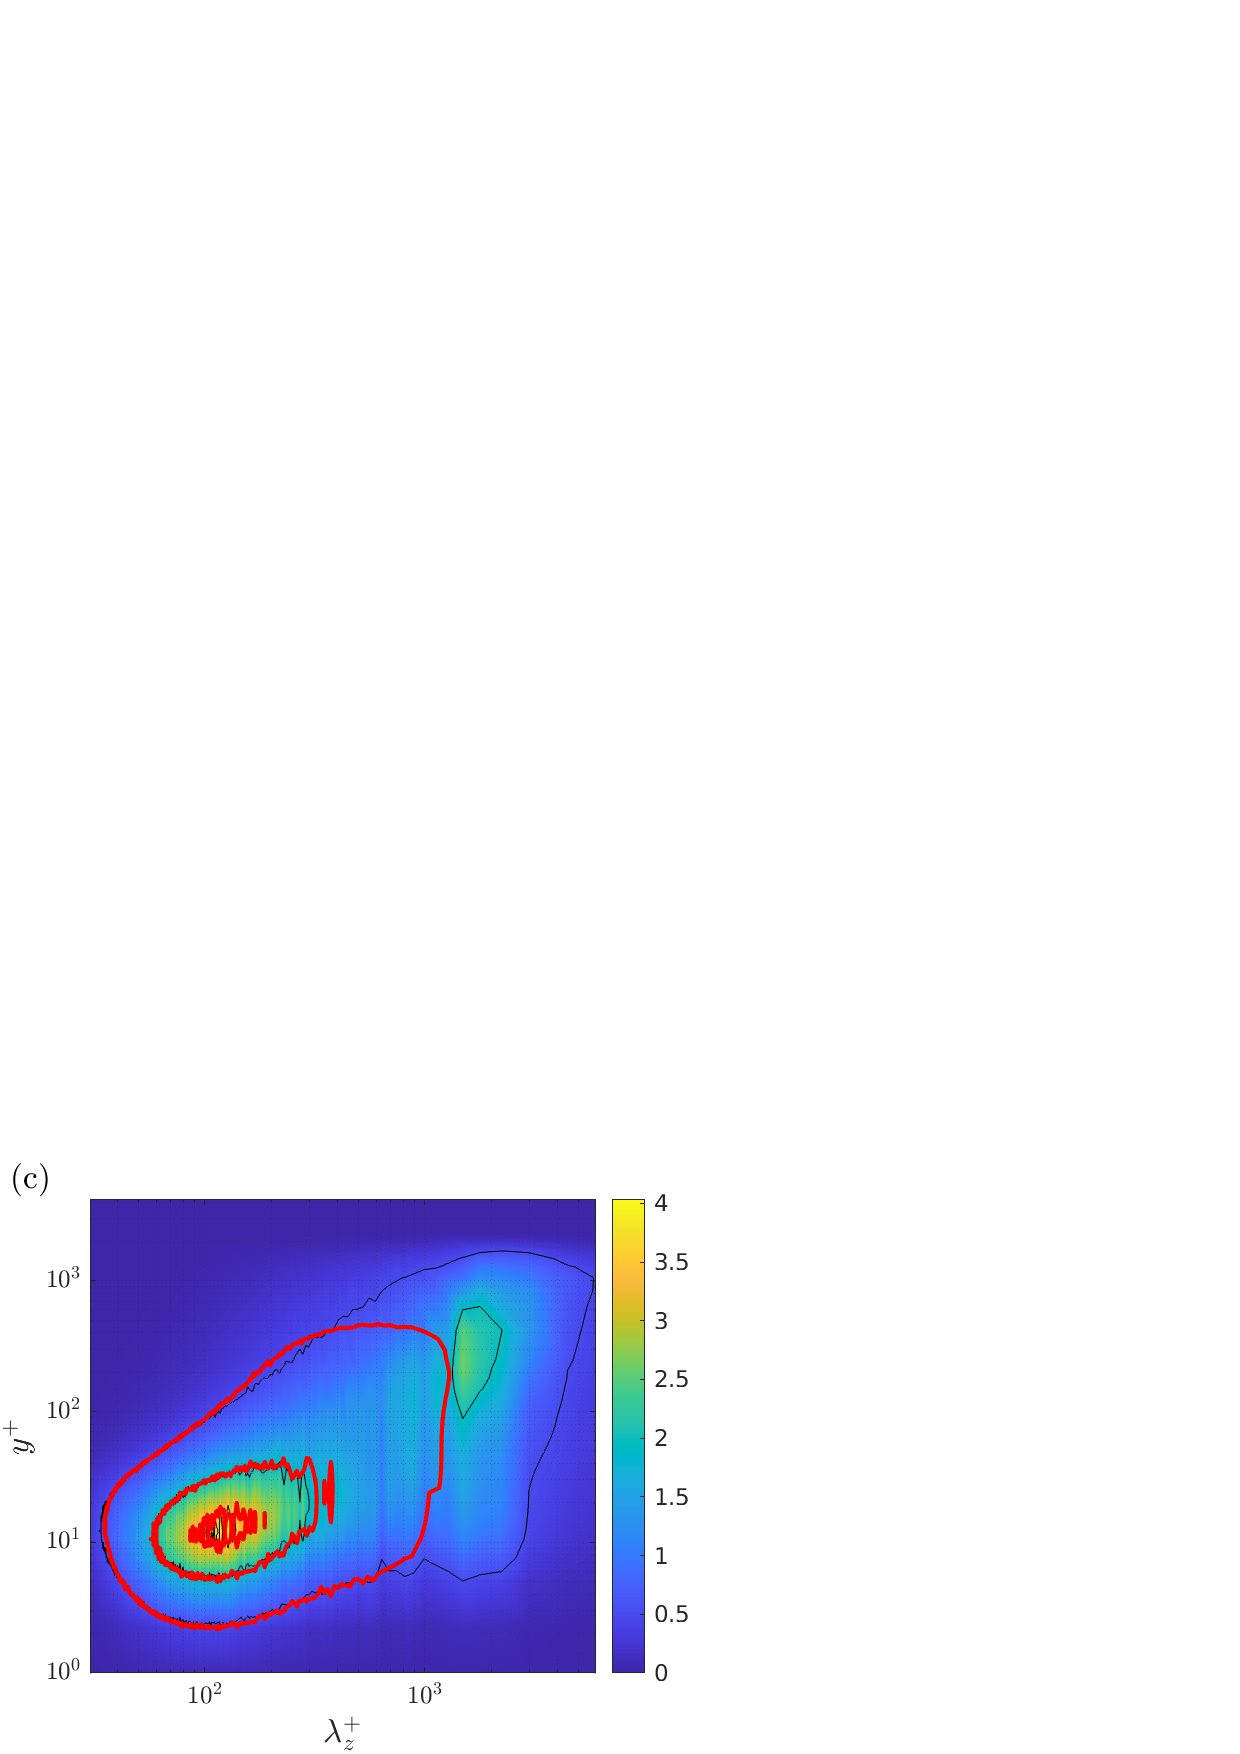
\includegraphics[width=0.32\textwidth]{imgs/spec/ZPG_Ret_500_2000_kPSdkz_lambdaz_ltau_y_ltau.jpg}
\caption{ \label{fig:PS_PSD} \highlight{ Spanwise spectra of the streamwise Reynolds stress $\overline{u\myprime ^2}(y)$ for a ZPG TBL, where the background and black contours represent a streamwise profile at $\Rey_{\tau}=2000$ and the red contours are taken at a position where $\Rey_{\tau}=500$.
(a) Power-spectral density $\phi_{u\myprime u\myprime}(y,k_z)$; (b) Power-spectral density $\psi_{u\myprime u\myprime}(y,\lambda_z)$; (c) premultiplied power spectral density $k_z\phi_{u\myprime u\myprime}(y,\lambda_z)$ (represented as a function of the wavelengths $\lambda_z=2\pi/k_z$). Wavenumbers, wavelengths, wall-normal position and power spectra scaled in viscous units.
}
}
\end{figure}
% contours: Retau 2000: [40 80  120 400 600]; [0.001 0.005 0.02 0.035 0.04] ;  [ 0.5 2 3.5]; 
% contours: Retau  500: [40 80  120        ]; [0.001 0.005 0.02 0.035 0.04] ;  [ 0.5 2 3.5]; 

The PS and the PSD in terms of the wavenumbers $\phi_{u\myprime u\myprime}(y,k_z)$ exhibit the same features as in Fig.~\ref{fig:PS_PSD}(a), since $\mathrm{d}k_z$ or $\mathrm{d}k_z^+$ are constant factors which do not vary with the wavenumbers. It shows a high content of power/energy of structures with a very low wavenumber, which are very wide. It is possible to see similarities in the contours at different Reynolds numbers (red and black lines) in the region of high wavenumbers (small scales), although the energetic level is very low compared to that of the low wavenumbers (large scales).
The PSD in wavelengths $\phi_{u\myprime u\myprime}(y,\lambda_z)$ is represented in Fig.~\ref{fig:PS_PSD}(b) and it focuses on the small scales. It shows that the density of power/energy in the small scales (short wavelengths) is very similar at different Reynolds numbers and larger than the PSD of the wider scales (large $\lambda_z^+$). 
From Fig.~\ref{fig:PS_PSD}(a) and (b) we see that the small scales have a small content of the total RS energy, but their small size makes their density in wavelength very concentrated, while for the wider scales it is the opposite, the energy they contain is very high, but their large size makes the PSD low.
If we write both PSDs as a function of $\phi_{u\myprime u\myprime}$, in Fig.~\ref{fig:PS_PSD}(a) we show $\phi_{u\myprime u\myprime}$ while in Fig.~\ref{fig:PS_PSD}(b) we present $k_z^2 \phi_{u\myprime u\myprime}$, and the premultiplication factor $k_z^2$ is responsible for enhancing the effects of the small scales while diminishing the effects of the large ones. Fig.~\ref{fig:PS_PSD}(c) shows $k_z \phi_{u\myprime u\myprime}$, whose effect equilibrates the effect of the large and small scales obtaining a better visualization of both scales.

The premultiplied PSD $k_z \phi_{u\myprime u\myprime}$ is widely used and it has a geometrical explanation.
Since the range of energetic scales is so large that we observe very small scales close to the wall and very large scales of the size of $\delta_{99}$, the use of logarithmic axes helps to expand the region of small $\lambda_z$ and the region close to the wall.
If we use logarithms in the definition of wavelength, $ \mathrm{ln}(\lambda_z) = \mathrm{ln}(2\pi) - \mathrm{ln}(k_z)$, apply the differential $\mathrm{d}(\mathrm{ln} \lambda_z) = -\mathrm{d}(\mathrm{ln} k_z)$, and consider $\mathrm{d}k_z = k_z \mathrm{d}(\mathrm{ln} k_z)$, we can substitute everything in Eq.~(\ref{eq:sum_ps}) to obtain:
\begin{equation}
    \overline{u_i\myprime u_j\myprime} = 
    \int_{k_0}^{k_{N}}   \phi_{u_i\myprime u_j\myprime}  ~ \mathrm{d} k_z = 
    \int_{k_0}^{k_{N}}   \phi_{u_i\myprime u_j\myprime} k_z  ~ \mathrm{d}( \mathrm{ln} k_z) = 
    \int^{\lambda_0}_{\lambda_{N}}   \phi_{u_i\myprime u_j\myprime} k_z ~ \mathrm{d}( \mathrm{ln} \lambda_z).
\end{equation}

The premultiplication by $k_z$ can be seen here as a factor to visualize a corrected area after scaling the axis with a logarithmic scale.
From here on the PSD will always be represented in its premultiplied form to provide a clear visualization of the effects of large and small scales at the same time.

\subsection{Wide scales in wall-bounded turbulence}
It has been shown that the large scales contain a significant fraction of the turbulent energy, although the spectral density is low.
When we model the turbulent flow, the size of the domain imposes a limit on the size of the scales that can be simulated. 
% In a periodic domain, the largest scale corresponds to $L_x$ and the wider scale to $L_z$. 
Scales larger than the domain will be seen as infinite in size because of the periodicity, and the spectral energy will be stored in the zero wavenumber. Note that the energy stored in this wavenumber is affected by the averaging.
If the size of the domain is not large enough, the larger turbulent scales will not be able to be represented in the domain and the energetic spectrum will not be correct, affecting the turbulence statistics.
Numerous studies on domain size have been performed on canonical turbulent channel flows due to their simplicity.
\highlight{Minimal channels are those small domains that assure }
On the other hand, the largest scales in channel flows were studied by ...
\highlight{CITAR ADRIAN que descubrieron bla bla}.
The study on the longest structures in $x$ was based on two-point correlations, but no other study similar to that of \highlight{CITAR ADRIAN} has been performed in the spanwise direction.

To achieve a better understunding of the wide scales obtained in APG TBLs and the effects of the domain size, we decided to study first the effect on wide channels.
Three simulations of turbulent channel flows at $\Rey_{\tau} = 550 $ were performed under similar conditions, with the only exception of the width of their domains, which was doubled from one channel to another as it can be seen in Table~\ref{tab:param_WC_cap2}.
 
\begin{table}
    \begin{center}
    \def~{\hphantom{0}}
    \begin{tabular}{ l c  c  c  r }
    Case  & $L_x/h$ & $L_y/h$ & $L_z/h$ &  Colour         \\[3pt]
    \hline
    C1    & 8$\pi$  &    2    & 4$\pi$  &  \WCblueline    \\
    C2    & 8$\pi$  &    2    & 8$\pi$  &  \WCredline     \\
    C3    & 8$\pi$  &    2    & 16$\pi$ &  \WCyellowline  \\
    \hline
    \end{tabular}
    \caption{Parameters of the channel-flow simulations. The reference length $h$ corresponds to the channel half height and the box size is $(L_x/h, L_y/h , L_z/h)$.}
    \label{tab:param_WC_cap2}
    \end{center}
\end{table}

\begin{figure}[h!]
\centering
% \captionsetup{width=0.99 \textwidth}
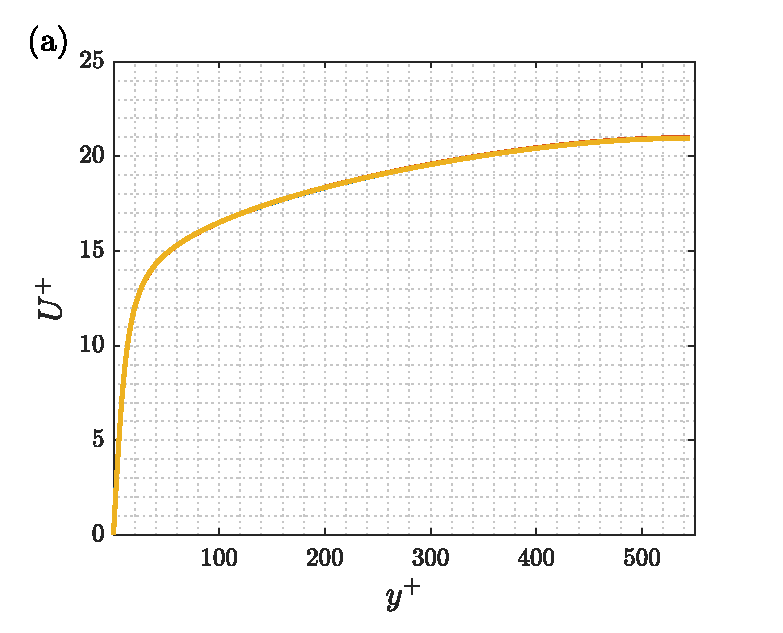
\includegraphics[width=0.49\textwidth ]{imgs/WC/U.eps}
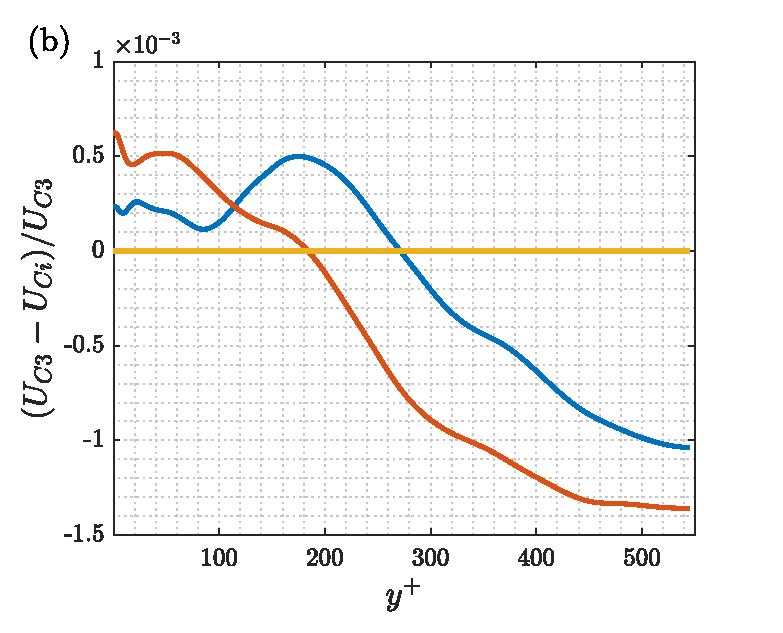
\includegraphics[width=0.49\textwidth]{imgs/WC/relerr_U.eps}
\caption{ \label{fig:WC_stats} (a) Mean streamwise velocity $U$ for channels C1 (blue), C2 (red) and C3 (yellow) scaled in viscous units.
(b) Relative error of $U$ with respect to the values for channel C3.}
\end{figure}
\begin{figure}[h!]
\centering
% \captionsetup{width=0.99 \textwidth}
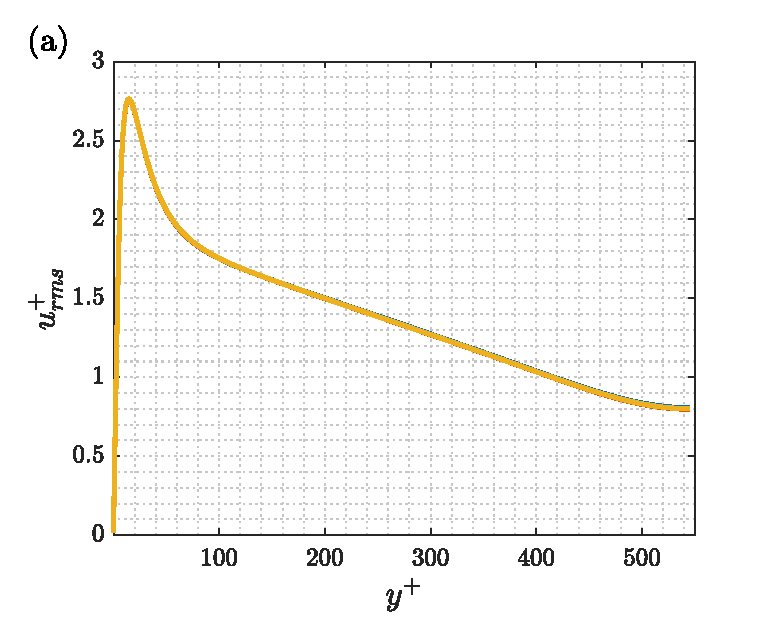
\includegraphics[width=0.49\textwidth]{imgs/WC/u_rms.eps}
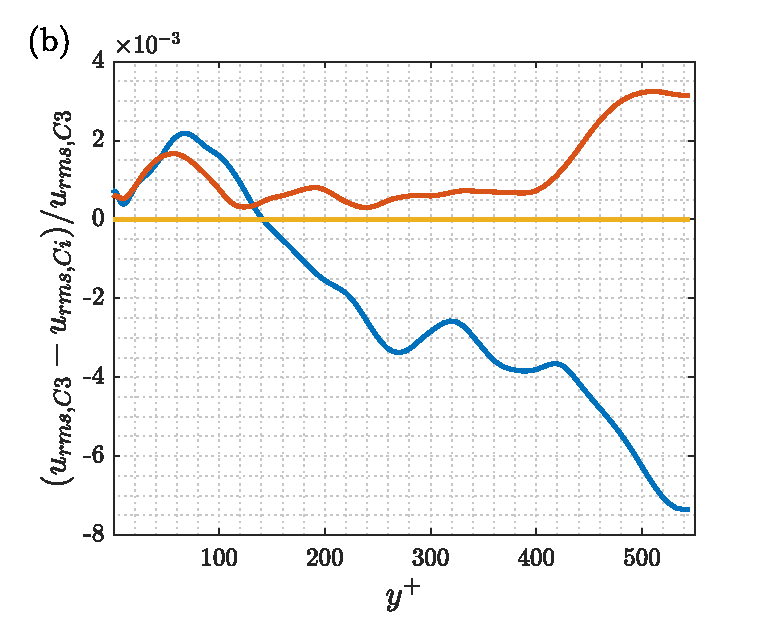
\includegraphics[width=0.49\textwidth]{imgs/WC/relerr_u_rms.eps}
\caption{ \label{fig:WC_stats} (a) Standard deviation $u_{rms}$ for channels C1 (blue), C2 (red) and C3 (yellow) scaled in viscous units.
(b) Relative error of $u_{rms}$ with respect to the values for channel C3.}
\end{figure}


\highlight{The contours of the PS or the spectral density $\phi(k_Z, y)$ are not closed for the largest scales when $k_z \rightarrow 0$. The largest scale captured by Fourier analysis corresponds to $k_Z=(2\pi)/L_z$ or $L_z$, and $k_z=0$ corresponds to an averaged energy. 
The property where the integral of the PSD equals the RS component includes the energy contained in the wavenumber $k_z=0$. The premultiplication by $k_z$ automatically cancels that energy, making it inappropriate to use premultiplied spectra for integral analysis. 
Then this question arises, ``is it possible to have a domain $L_z$ where the largest Fourier scales $\lambda_z=\{L_z, L_z/2, ... \}$ does not contain spectral energy, therefore the contours are closed?''.
And the answer is that it depends on the averaging that we use. This answer will be explained using the Reynolds-average decomposition that we have introduced previously, and apply it to the component $u$.}
With $PS_T$ we denote the power spectra of the total velocity $u$, and the energy contained in the wavenumber $k_z$ corresponds to the average in $z$.


\begin{equation}
    PS_T = \mathcal{F}(u)\mathcal{F}^*(u) = \mathcal{F}(U)\mathcal{F}^*(U) + \mathcal{F}(u\myprime)\mathcal{F}^*(u\myprime) + \mathcal{F}(U)\mathcal{F}^*(u\myprime) + \mathcal{F}(u\myprime)\mathcal{F}^*(U)  
\end{equation}

\begin{flalign}
    % \label{eq:intsc_3term_small}
     PS_T =& \mathcal{F}(u)\mathcal{F}^*(u) &&\\\nonumber
     =&  \mathcal{F}(U)\mathcal{F}^*(U) + \mathcal{F}(u\myprime)\mathcal{F}^*(u\myprime) + \mathcal{F}(U)\mathcal{F}^*(u\myprime) + \mathcal{F}(u\myprime)\mathcal{F}^*(U) &&\\\nonumber
     =&  UU + \mathcal{F}(u\myprime)\mathcal{F}^*(u\myprime) + U(\mathcal{F}(u\myprime) + \mathcal{F}^*(u\myprime)) &&\\\nonumber
\end{flalign}  
\rev{and the last term vanishes when the time average is performed?}

\begin{equation}
\begin{split}
    % \label{eq:intsc_3term_small}
     PS(k_z=0,t) = \langle u\myprime \rangle_z \langle u\myprime \rangle_z  (t) \\
     \langle PS(k_z=0) \rangle_t = \langle (\langle u\myprime \rangle_z)^2 \rangle_t > 0,
\end{split}
\end{equation}
since by definition, $U$ and $u\myprime$ are chosen as a constant and a fluctuation based on the total average $\overline{( \cdot )} = \langle \langle ( \cdot ) \rangle_z \rangle_t$, and $\overline{u\myprime}=0$, but $ \langle u\myprime \rangle_z \neq 0$.

Therefore, the energy contained in $k_z=0$ can not be 0, but it is somehow a result of the average used for the decomposition.
What can be study is how the energy contained in $k_z=0$ changes with $L_z$, and even more relevant from the physical point of view is how much is the energy contained in the first wavenumbers or the largest scales $\lambda_z=L_z, L_z/2, L_z/3,...$.


\subsection{Spectral analysis of APG TBLs}

In \textbf{Paper 1} the 1D spanwise spectra and the 2D spanwise and temporal spectra of the APG TBL where shown and compared with those of a ZPG TBL \citep{EAmorZPG}. By using percentage contours it was possible to show a similar behaviour in the mild APG and the ZPG simulations at different Reynolds numbers in the small-scale energy region close to the wall around an spectral near-wall peak or spectral inner peak (sIP) at $y^+\approx 15$ and $\lambda_z^+\approx 120$. Another region with similar shape is the wake region, which exhibits an spectral outer peak that appears to scale with Reynolds number.
Another region is that of small-scale energy in the wake region, which is only present in the APG simulation and not in the ZPG case.

\begin{figure}[h!]
\centering
% \captionsetup{width=0.99 \textwidth}
\includegraphics[width=0.48\textwidth]{ZPG_uu.jpg}
\includegraphics[width=0.48\textwidth]{APG_uu.jpg}
% 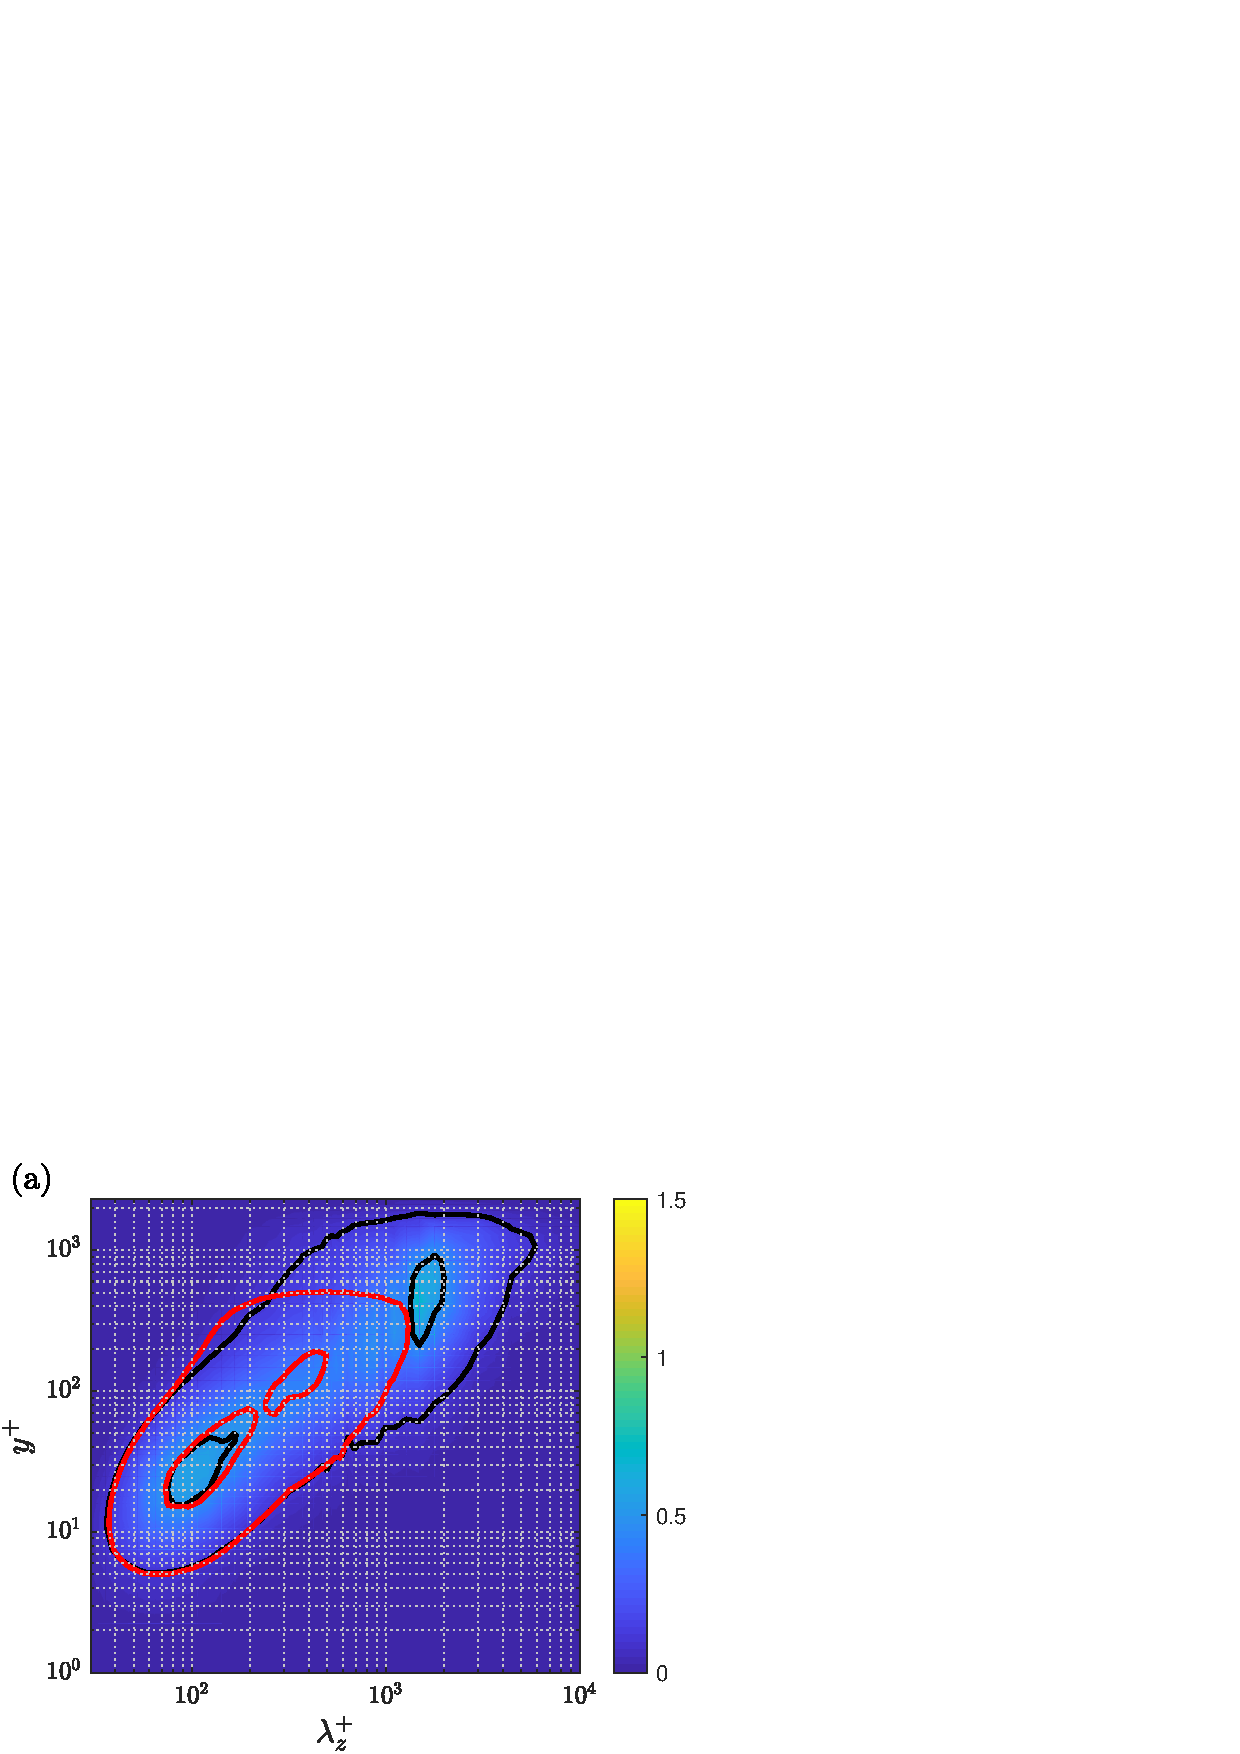
\includegraphics[width=0.48\textwidth]{ZPG_uv.jpg}
% 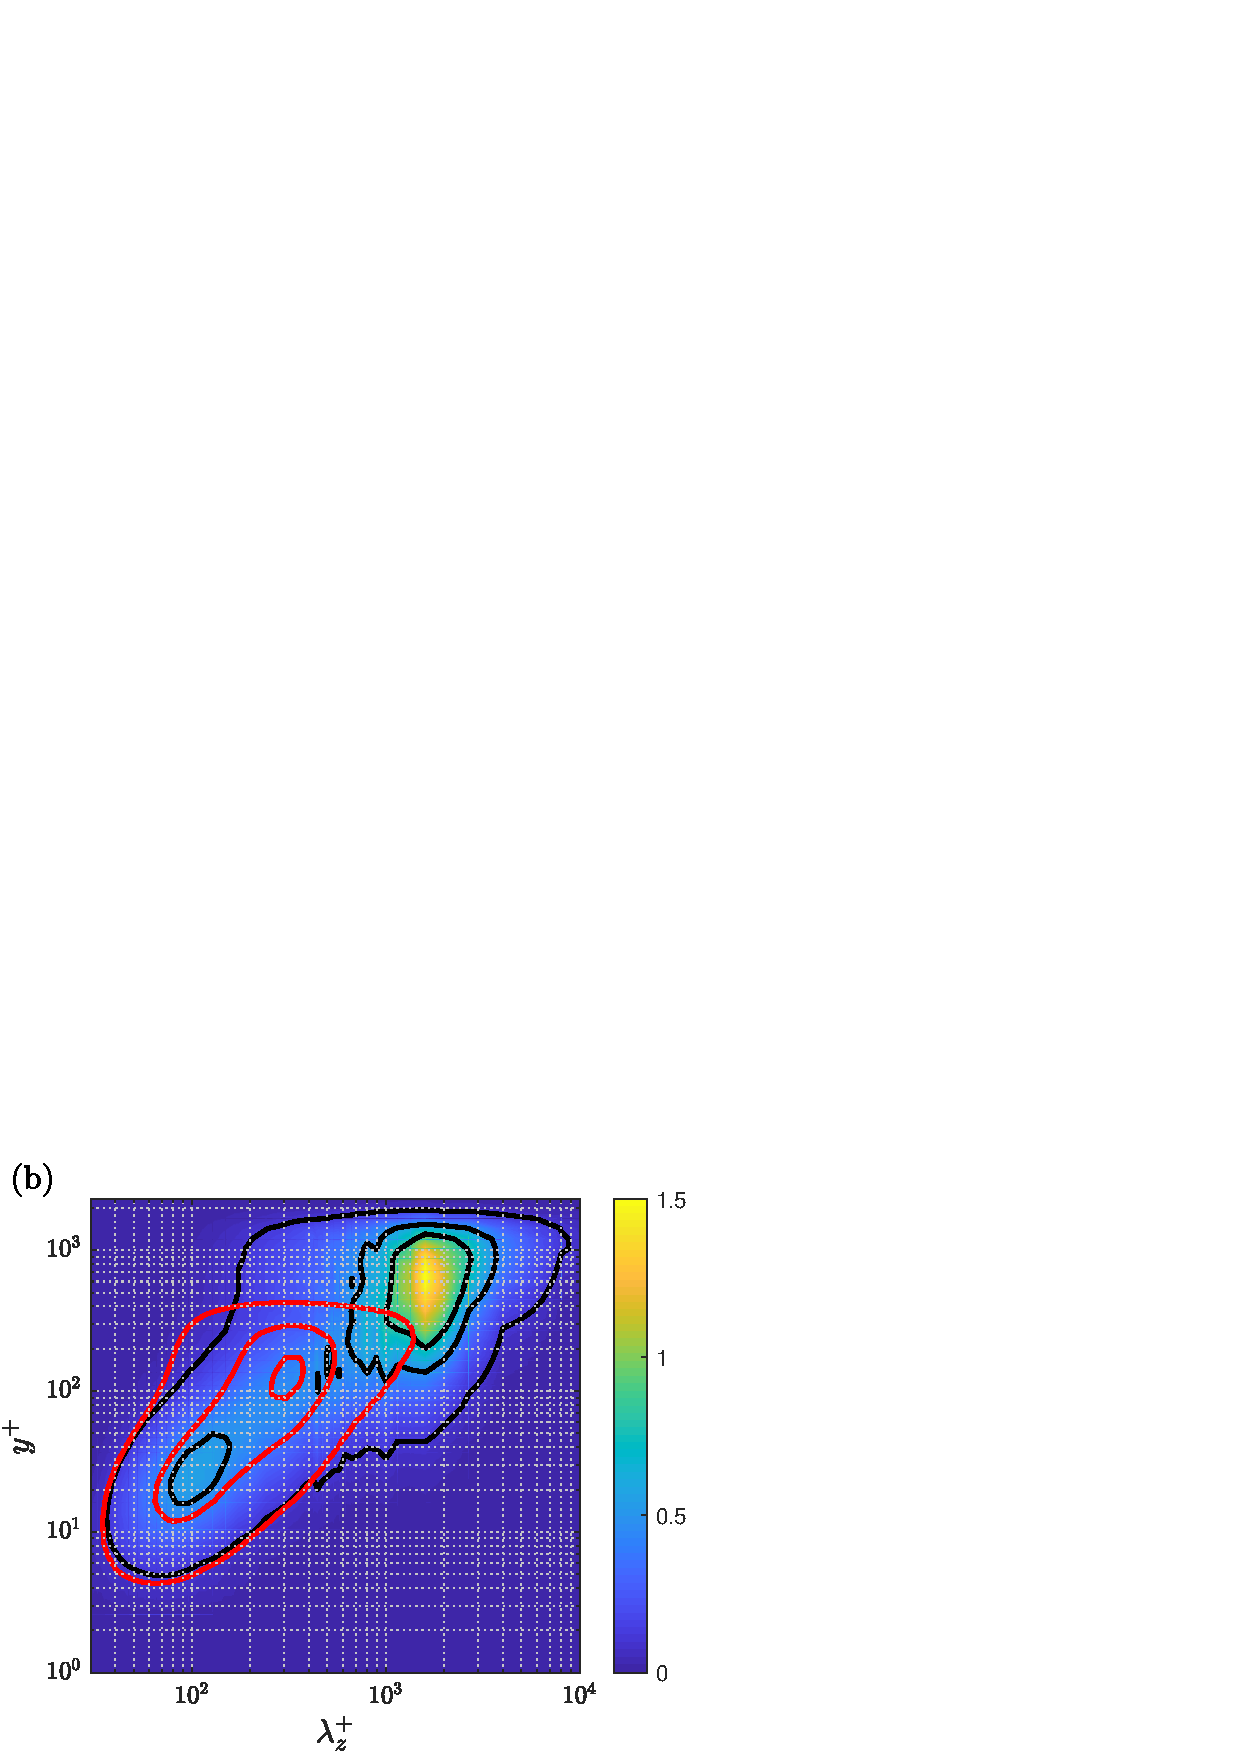
\includegraphics[width=0.48\textwidth]{APG_uv.jpg}
\caption{ \label{fig:ZPG_APG_Ret_500_2000_uu} Premultiplied spectrum $k_z\phi_{uu}$ for (a) ZPG and (b) b1.4 simulations. Red contours at $\Rey_{\tau}=500$, background and black contour are at $\Rey_{\tau}=2000$. }
\end{figure}

\begin{figure}[h!]
\centering
% \captionsetup{width=0.99 \textwidth}
% \includegraphics[width=0.48\textwidth]{ZPG_uu.jpg}
% \includegraphics[width=0.48\textwidth]{APG_uu.jpg}
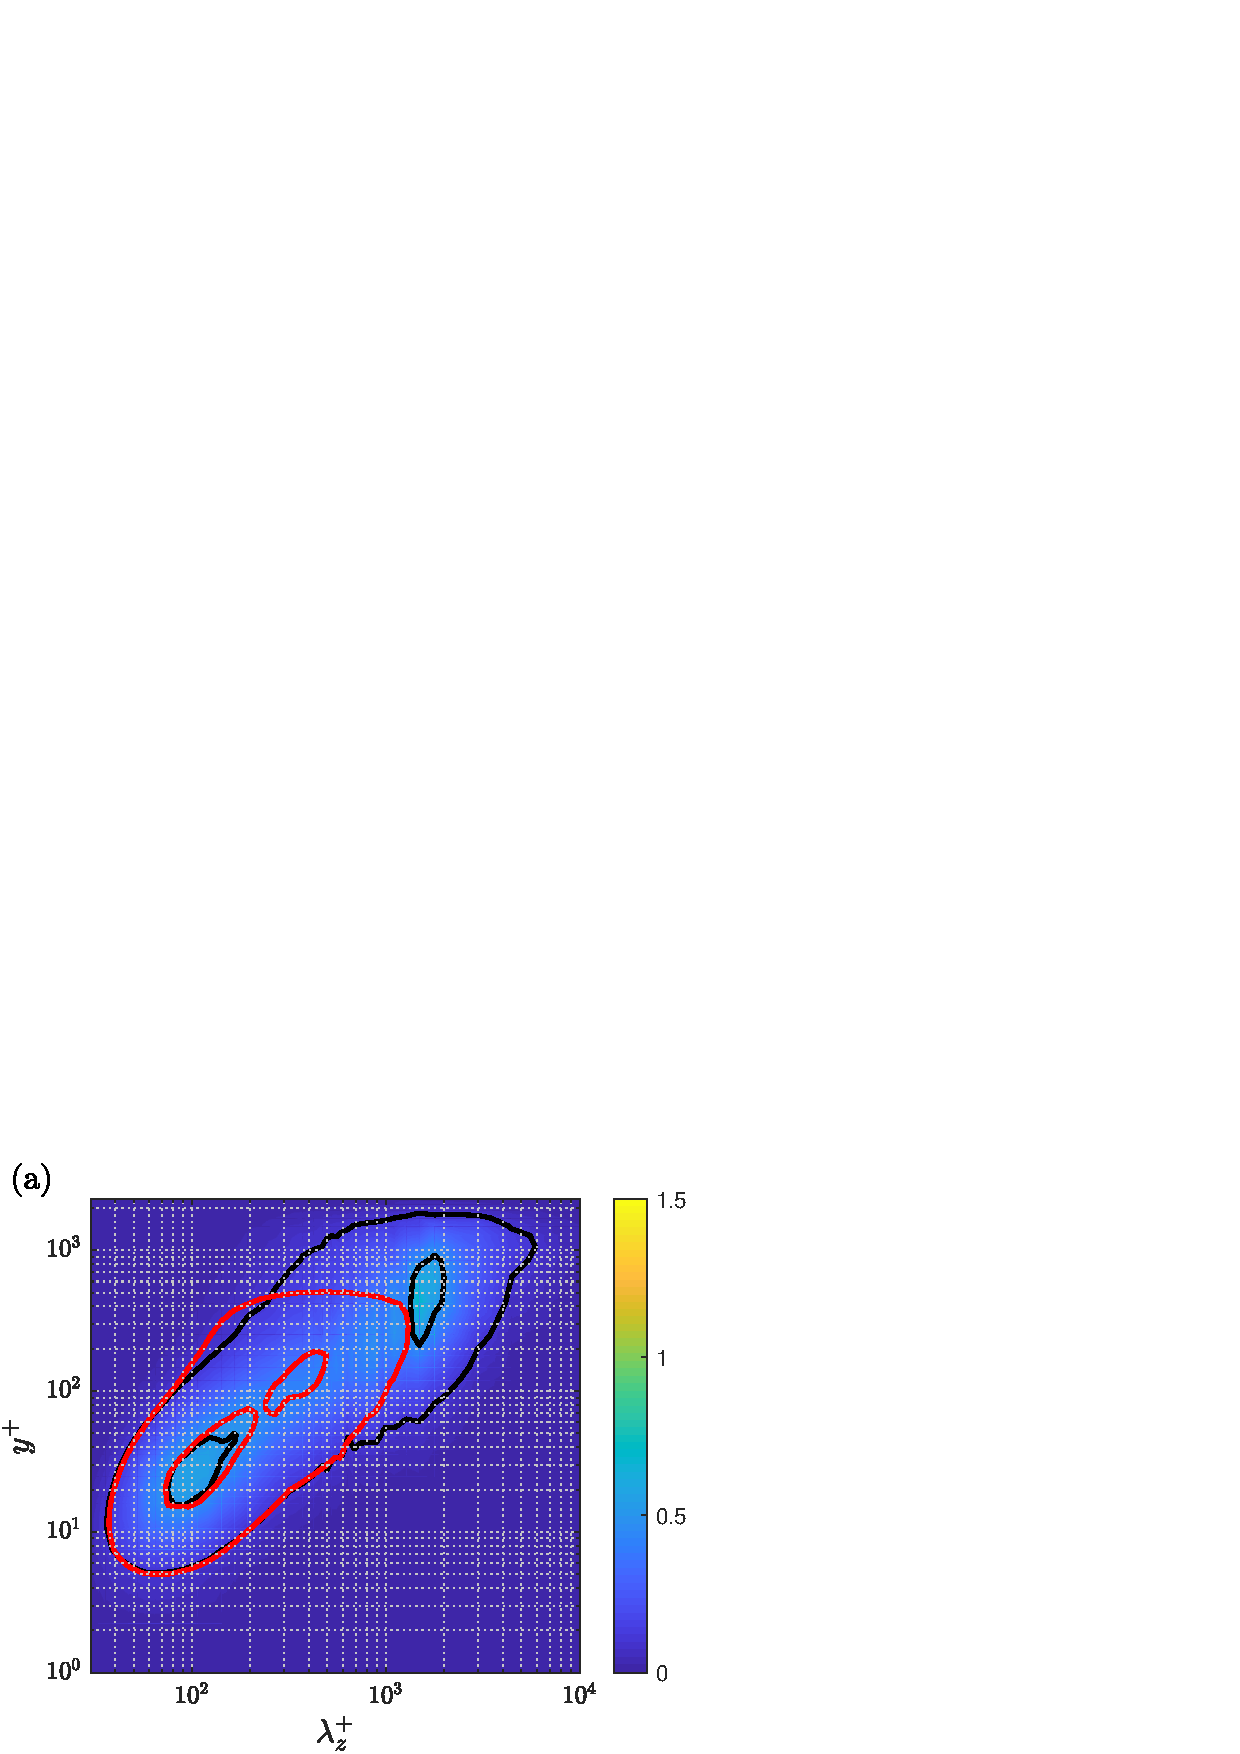
\includegraphics[width=0.48\textwidth]{ZPG_uv.jpg}
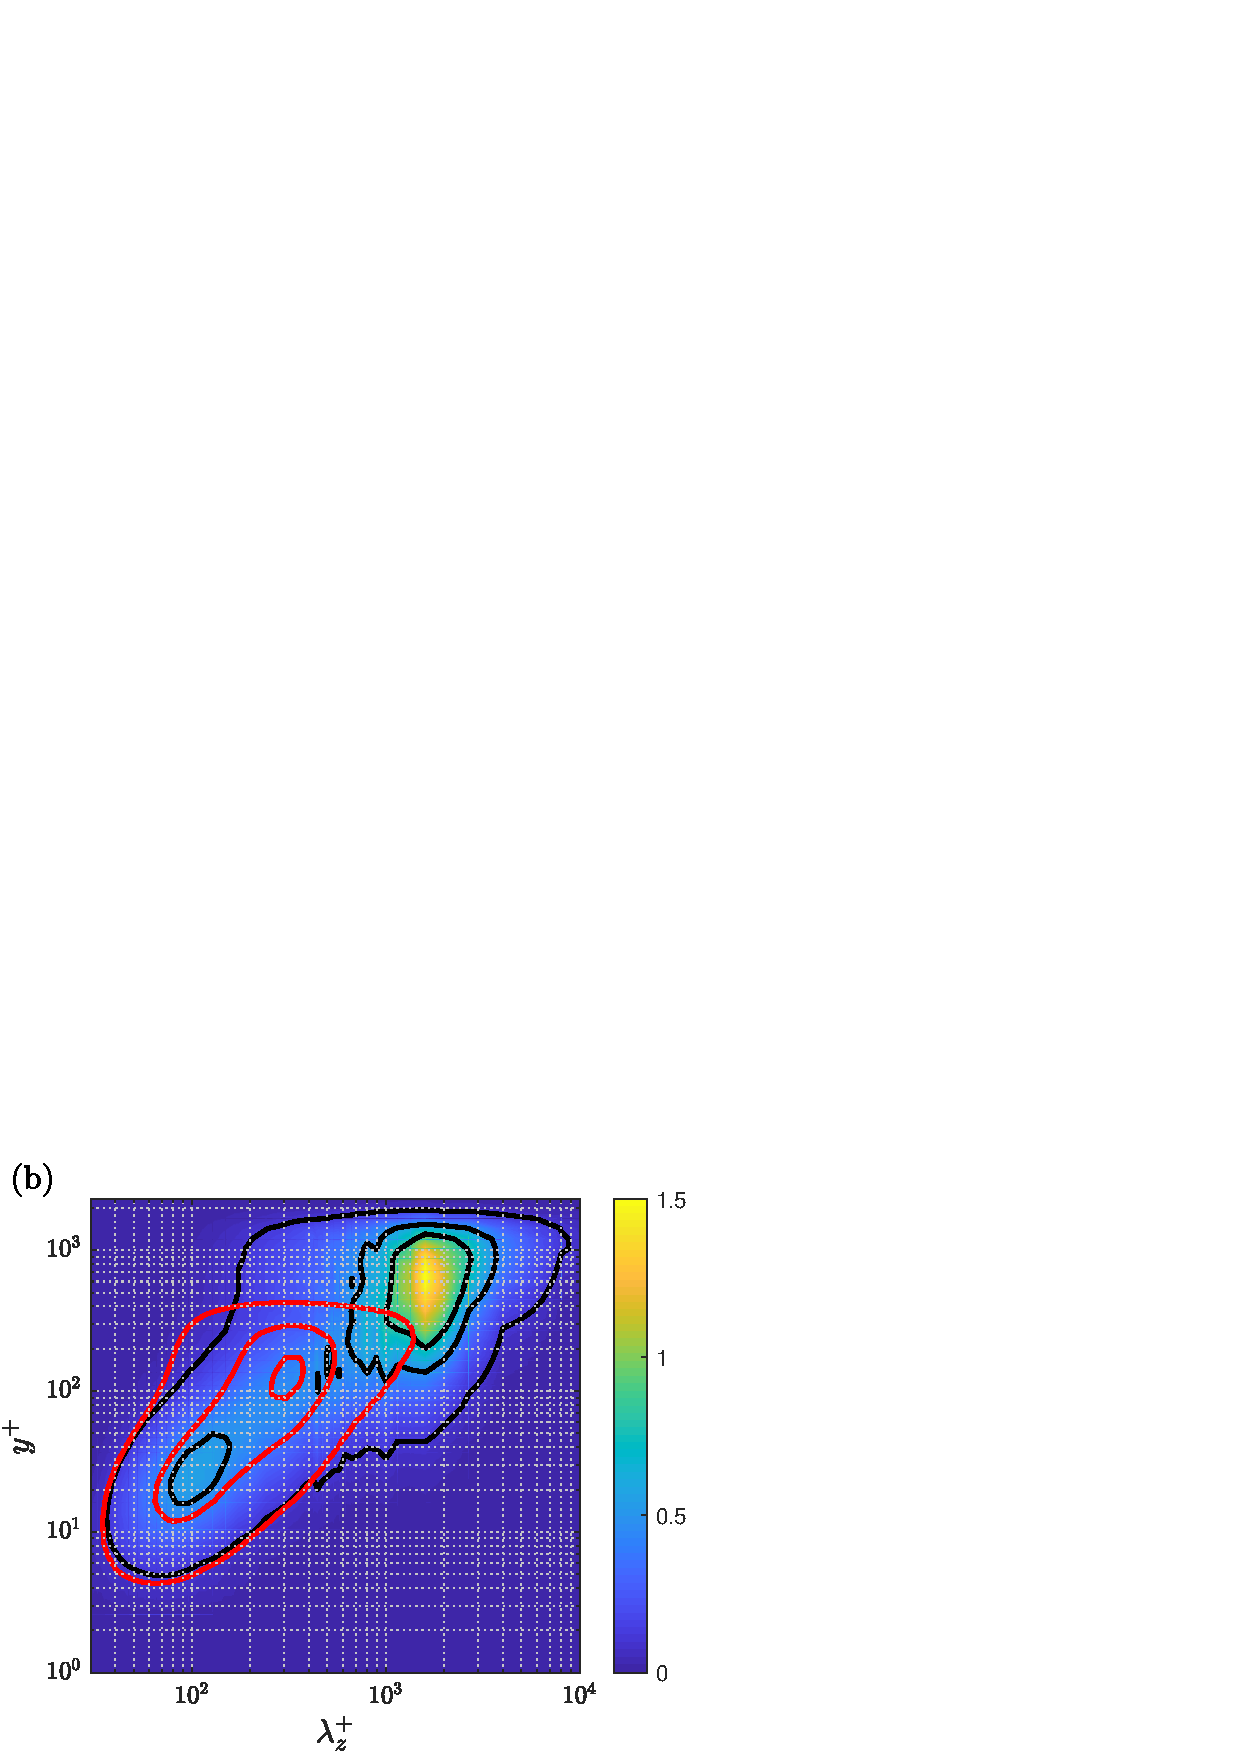
\includegraphics[width=0.48\textwidth]{APG_uv.jpg}
\caption{ \label{fig:ZPG_APG_Ret_500_2000_uv} Premultiplied cospectrum $|k_z\phi_{uv}|$ for (a) ZPG and (b) b1.4 simulations. Red contours at $\Rey_{\tau}=500$, background and black contour are at $\Rey_{\tau}=2000$. }
\end{figure}

The spectra exhibit a similar region of small-scale energy close to the wall which is responsible of the near-wall peak of $\overline{u\myprime^2}$. The effects of $\Rey$ and $\beta$ increase the value of $\overline{u\myprime ^2}_{\rm IP}^+$, even if a significant fraction of the spectrum is similar for APG and ZPG at different Reynolds numbers.
The outer spectral peak in $k_z\phi_{uu}$ is also responsible for most of the energy contained in the ZPG in the wake region, and increasing $\beta$ raises the energy to the point of developing an outer peak in $\overline{u\myprime^2}_{OP}^+$. This behaviour is similar in the other components of the RS tensor, where at higher $\Rey$ there are larger and energetic scales acting on the wake region and influencing all across the TBL.

\subsection{Scaling of APG spectrum}

In \textbf{Paper 2} we try to understand the trends of the inner and outer peaks in $\overline{u\myprime ^2}$ shown in \textbf{Paper 1}. First, we assess why the inner-scaled inner peak grows with Reynolds number and APG magnitude. 
We perform a scaling analysis of the different energetic scales of the power-spectral density for both ZPG and APG simulations and at different Reynolds numbers.
First we start from the features observed in $k_z\phi_{u\myprime u\myprime}$ which are the spectral near-wall/inner peak (sIP) and the spectral outer peak (sOP). 
% The data is scanned to look for the maxima at a certain wall-normal position and the maxima at a certain frequency. Since $k_z\phi_{u\myprime u\myprime}$ is saved in a rectangular matrix, it is equivalent to obtain the maxima along columns and the maxima along rows.
At high Reynolds number the separation of scales, allows to clearly distinguish the presence of 2 maxima points for $\Rey_{\tau}>500$. 
% Other techniques could be used to detect the local maxima, but this method was obtaining satisfactory results, specially the values of $f(y)=max(k_z\phi(k_z, y))_{k_z}$ since that function presents less noise and it is shown in \highlight{ Fig.~\ref{fig:scaling_OP} figura de los escalados de los picos} that once the Reynolds number is enough to have separation of scales, the outer peak clearly separates in the wall-normal direction from the spectral near-wall peak.
Our results show that for high enough $\Rey$ we observe sufficient separation of scales so that the outer peak clearly separates in the wall-normal direction from the spectral near-wall peak.
Once sIP and sOP are located in $k_z\phi(k_z, y)$, (it is usually represented as a function of $\lambda_z$), we try the inner and outer length scalings used in \textbf{Paper 1} to scale $\overline{u\myprime ^2}(y)$.
Our results show that the viscous length $\ell_{\tau}$ scales the size of the spanwise scales of the sIP $\lambda_{z, \mathrm{sIP}}^+$ as well as the wall-normal position $y^+_{\mathrm{sIP}}$.
The same method is used for the spectral outer peak. The outer scales $\delta^*$ and $\delta_{99}$ were used to scale independently the wall-normal location $y_{\mathrm{sOP}}$ and the size of the scales $\lambda_{z, \mathrm{sOP}}$.
In previous studies such as that by \cite{Kitsios2017} the $\delta^*$ scaling was successful for the $y_{\mathrm{OP}}$ as well as for $y_{\mathrm{sOP}}$ at much higher $\beta$, however, $\lambda_z$ was also scaled with the same scaling.
In \cite{tanarro_2020}, the outer scaling was performed with $\delta_{99}$ for both $y$ and $\lambda_z$, and the values of $\lambda_{z,\mathrm{sOP}}$ collapsed better than using $\delta^*$ as in \cite{Kitsios2017}.
Taking into account these previous studies, we allowed $y$ and $\lambda_z$ to have different length scalings, and found the optimal collapse of the region around the spectral outer peak using $y/\delta^*$ and $\lambda_z/\delta_{99}$.

Once we obtained the scalings for the wall-normal position and size of the scales for both sIP and sOP, we analyzed the region around those peaks using the respective scalings, obtaining a good collapse. However, there was another region to investigate, which is the area of small-scale energy in the wake region.
Different scalings were tried for $\lambda_z$ with the aim of collapsing the vertical part of the energetic contours of the APG simulation at different $\Rey$.
We observed that using $\lambda_z/\delta^*$ there is a collapse around $\lambda_z/\delta^*=0.3$. It could be argued that the scaling evolves gradually at different $\lambda_z$ up to the region around the sOP that clearly scales using $\lambda_z/\delta_{99}$.
To have a better idea of how big was the contribution of the small-scale energy in the wake region, but also to understand what is the influence of the large scales in the near-wall region, we accumulated the energy from small to large scales for all the wall-normal positions. In a matrix containing the $\mathrm{PS}(y,k_z)$, this is equivalent to doing a cumulative sum $\text{cumsum}(\mathrm{PS}(y,k_z))_{k_z}$ along $k_z$.
In \cite{EAmorZPG}, they performed this on a rectangular region around the sIP, to show that inner-scaled energy in this region does not vary with the Reynolds number, but we have seen that there are different scalings at different wall-normal locations in the TBL. Thus, the rectangular domain to integrate over $\lambda_z$ and $y$ may not be the optimal tool for this analysis.

With the idea of looking for the contribution of small and large scales using a cumulative sum, and conjecturing that the accumulated energy would exhibit some that probably would change with $\Rey$ effects, we proposed the percentual contribution of energy, or the marginal contribution of energy.
For a continuous PSD, the marginal contribution of energy (MCE) is defined as in Eq.~(\ref{eq:MCE_cap2}) and yields the percentual level of energy from the scales up to a wavenumber $k_{z,c}$ with respect to the total value, which would be $\overline{u_i\myprime u_j\myprime}$ at that particular $y$.

\begin{equation}
\mathrm{MCE} = \int_{k_{z,c}}^{\infty} \phi_{u_iu_j} \mathrm{d} k_z \ \bigg/ \int_{0}^{\infty} \phi_{u_iu_j} \mathrm{d} k_z.
\label{eq:MCE_cap2}
\end{equation}

By analyzing different contour levels, it is possible to study the regions where certain choices of length and energy scales are valid, since the contours will be parallel where the scales contribute in the same way to the total RS. And they will start to diverge when the scaling is not appropriate.
Where the scaling is independent of $\Rey$, the contours for different $\Rey$ at the same MCE level in that region will collapse, otherwise they will start to separate indicating for example that the influence of large-scale motions is affecting that region.
\highlight{
In Fig.~\ref{fig:MCE_spec}(a), we can see the region of influence of the viscous scaling, where the blue lines show scales smaller than those of the sIP have a similar percentual relevance with $\Rey$ and $\beta$; the green parallel lines scale in viscous units for both ZPG and APG simulations, although they are separated because of the APG largest scales being more relevant than in the ZPG case.
The outer peak region is show in Fig.~\ref{fig:MCE_spec}(b) and is characterised by spanwise scales $\lambda_z$ which scale with $/\delta_{99}$ in a wall-normal region that scales with $\delta^*$.
The small-energy scales active in the outer region are seen to be scaled with $\lambda_z/\delta^*$ in Fig~\ref{fig:MCE_spec}(c).
}
All of this is shown in \textbf{Paper 2} in more detail.
Regarding the question of why $\overline{u\myprime ^2}_{IP}^+$ grows with $\Rey$ and $\beta$, at higher $\Rey$ the influence of scales 
\highlight{
$\lambda_z \geq \delta_{99}$ affects the near-wall region, the dark-red contours show the larger influence of large scales with $\Rey$ for the ZPG case. The lighter-red contours show the same behaviour in the APG case, where the larger scales are even more relevant than in the ZPG case.
}
In this range of $\beta$ the viscous scaling is still valid, although some modifications could be done taking into account the influence of the large scales.
At larger $\beta$, the flow approaches separation and the viscous scaling is no longer applicable.

\begin{figure}[h!]
\centering
% \captionsetup{width=0.99 \textwidth}
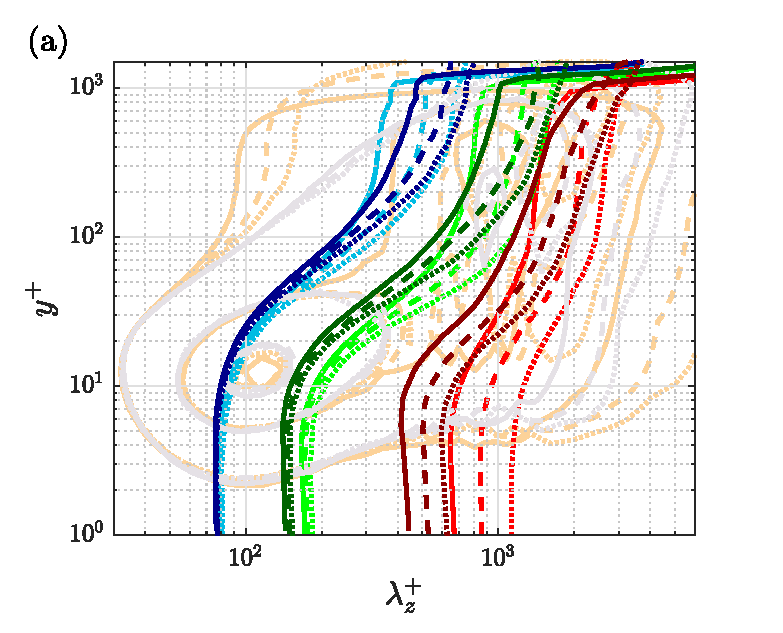
\includegraphics[width=0.45\textwidth]{imgs/spec/specMCE_uu_ltau_ltau.eps}
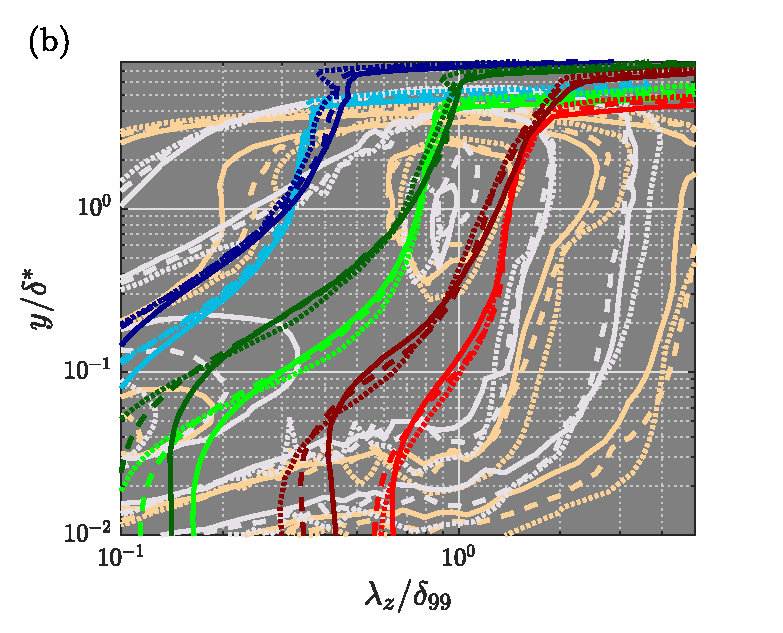
\includegraphics[width=0.45\textwidth]{imgs/spec/specMCE_uu_dstar_d99.eps}
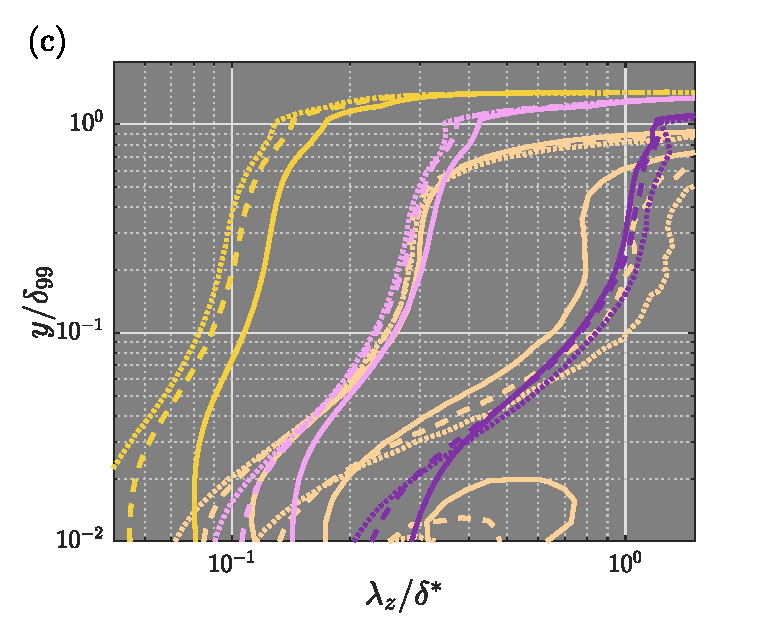
\includegraphics[width=0.45\textwidth]{imgs/spec/specMCE_uu_d99_dstar.eps}
\caption{ \label{fig:MCE_spec}
\highlight{ 
Contours of the premultiplied spectra $k_z\phi_{uu}$ in orange for b1.4 and light gray for the ZPG simulations.
The blue($20\%$), green($50\%$) and red($80\%$) lines are the MCE contours, where the light colors are used for the APG and the darker shades for the ZPG case.
Solid lines are used for $\Rey_{\tau}=1000$, dashed lines for $\Rey_{\tau}=1500$ and dotted lines $\Rey_{\tau}=2000$. Panel (a) shows the region that scales using inner scaling for both $y$ and $\lambda_z$; (b) scales the larger scales in the wake region by using two different length scales, $y\delta^*$ and $\lambda_z/\delta_{99}$. Panel (c) shows the scaling of the small-scale energy in the wake region characteristic of APGs, where $\lambda_z$ scales with $\delta^*$. The MCE contours are taken at $0.1\%$(yellow), $2.2\%$(pink) and  $15\%$(purple). 
}
}
\end{figure}





